\documentclass[14pt,a4paper]{article}

\usepackage[russian]{babel}
\usepackage{hyperref}
\usepackage{indentfirst}
\usepackage{float}
\usepackage{geometry}
\usepackage{graphicx}
\usepackage{verbatim}
\usepackage{wrapfig}
\usepackage{qtree}

\setlength{\parindent}{0.5cm}
\geometry{top=2cm, bottom=2cm, left=1.5cm, right=1.5cm}
\renewcommand{\thesubsection}{\arabic{subsection}}
\renewcommand{\labelenumi}{\arabic{enumi})}  
\newcommand{\customtitle}[2]{%
\begin{titlepage}
  \begin{center}
    {\large\scshape\bfseries
    МИНИСТЕРСТВО НАУКИ И ВЫСШЕГО ОБРАЗОВАНИЯ РОССИЙСКОЙ ФЕДЕРАЦИИ\\
    ФЕДЕРАЛЬНОЕ ГОСУДАРСТВЕННОЕ АВТОНОМНОЕ ОБРАЗОВАТЕЛЬНОЕ УЧРЕЖДЕНИЕ ВЫСШЕГО
    ОБРАЗОВАНИЯ\\
    «СЕВЕРО-КАВКАЗСКИЙ ФЕДЕРАЛЬНЫЙ УНИВЕРСИТЕТ»\\
    ФАКУЛЬТЕТ МАТЕМАТИКИ И КОМПЬЮТЕРНЫХ НАУК ИМЕНИ ПРОФЕССОРА Н.И.ЧЕРВЯКОВА}
    \vfill
    \Large{\textbf{ЛАБОРАТОРНАЯ РАБОТА №#1}}\\[2mm]
    \large{Алгоритмизация и программирование}\\[6mm]
    \large{\textbf{#2}}\\[20mm]
  \end{center}
  \begin{flushright}
    \large{
      \textbf{Выполнил студент:}\\
      Сивко Иван Андреевич\\
      студент 2 курса\\
      группа ПМИ-б-о-23-2,\\
      направление подготовки 01.03.02\\[5mm]
      \textbf{Проверил:}\\
      Ассистент кафедры вычислительной\\
      математики и кибернетики, к.ф.-м.н.,\\
      Черкашина Анастасия Андреевна}
  \end{flushright}
  \vfill
  \centerline{ \the\year\ г. }
\end{titlepage}
    }

\newenvironment{fancyblock}
  {\large\bfseries\scshape}
  {}

\begin{document}
\customtitle{21}{Классы}
\large{\textbf{
\centerline{Вариант 9}
Цель:
}
\begin{small}
  \begin{itemize}
    \item Совершенствование навыков разработки программ в среде программирования MS Visual C++
    \item Совершенствование навыков в программировании с использованием модульного подхода
  \end{itemize}
\end{small}
\section*{Задание 1}
\subsection{Условие:}
Составить описание класса для определения одномерных массивов строк фикси­рованной длины. Предусмотреть следующие возможности:
\begin{itemize}
  \item обращение к отдельным строкам массива по индексам;
  \item контроль выхода за пределы массива;
  \item выполнение операций поэлементного сцепления двух массивов с образованием нового массива;
  \item слияния двух массивов с исключением повторяющихся элементов;
  \item вывод на экран элемента массива по заданному индексу и всего массива.
\end{itemize}
Написать программу, демонстрирующую работу с этим классом.
\subsection{Алгоритм / Мат. модель}
Программа использует класс, предназначенный для работы с одномерными массивами
строк фиксированной длины. Класс поддерживает различные операции с массивами
строк, такие как обращение к отдельным строкам, сцепление массивов, слияние с
исключением дубликатов и вывод на экран. Все операции с массивами контролируют
выход за пределы массива и выполняют необходимые действия для предотвращения
ошибок. Программа демонстрирует работу с этим классом и позволяет эффективно
управлять строками в массиве.
\begin{enumerate}
  \item \textbf{Инициализация структуры данных:} Создается класс \texttt{CArrWrapper}, который инкапсулирует массив строк. Каждое строковое поле представляет собой объект \texttt{CStrWrapper}, хранящий строку.
    \begin{itemize}
      \item \texttt{size\_} — количество элементов в массиве (строк),
      \item \texttt{data} — указатель на массив строк типа \texttt{T*},
      \item \texttt{CArrBase<T>} — базовый класс, предоставляющий общие методы для работы с массивом: доступ к элементам по индексу, операции с памятью.
    \end{itemize}
  \item \textbf{Обращение к строкам массива:} Массив строк поддерживает доступ к отдельным элементам по индексу с помощью оператора \texttt{[]}. При попытке доступа к несуществующему элементу генерируется исключение.
  \item \textbf{Контроль выхода за пределы массива:} Для предотвращения выхода за пределы массива, при обращении к элементам используется проверка \texttt{assert(idx < size\_)} для гарантии, что индекс находится в пределах допустимого диапазона.
  \item \textbf{Сцепление двух массивов:} Операция сцепления двух массивов строк выполняется через оператор \texttt{+=}, что приводит к созданию нового массива, содержащего элементы обоих исходных массивов. При этом формируется новый объект класса \texttt{CStrWrapper}, в который добавляются элементы из обоих массивов.
  \item \textbf{Слияние массивов с исключением повторяющихся элементов:} Функция \texttt{mergeUnique} сливает два массива строк, исключая повторяющиеся элементы. Для каждого элемента второго массива осуществляется проверка наличия его в первом массиве. Если элемент не найден, он добавляется в новый массив.
  \item \textbf{Вывод массива:} Функция \texttt{operator<<} выводит все элементы массива на экран в виде списка, разделенного запятыми. Каждый элемент массива отображается по порядку.
  \item \textbf{Реализация через командную строку:} Программа создает два массива строк, выполняет их слияние с исключением повторов, а затем выводит результат на экран.
\end{enumerate}
\fbox{
  \parbox{0.8\textwidth}{
      \textbf{Дерево наследования} \\[10pt]
    \begin{center}
      \Tree
      [.CArrBase
      [.CArrWrapper ]
      [.CStrWrapper ]
      ]
    \end{center}
  }
}

\begin{table}[H]
  \centering
  \begin{tabular}{|l|l|} \hline
    \textbf{Член класса} & \textbf{Описание} \\ \hline
    size\_ & Размер массива (количество элементов) \\ \hline
    data & Указатель на массив данных (тип T*) \\ \hline
    \textbf{Метод класса} & \textbf{Описание} \\ \hline
    CArrBase(size\_t, T*) & Конструктор, инициализирующий размер и данные массива \\ \hline
    CArrBase() & Конструктор по умолчанию (неинициализированный массив) \\ \hline
    CArrBase(size\_t) & Конструктор, выделяющий память для массива указанного размера \\ \hline
    \textasciitilde CArrBase() & Деструктор, освобождает память массива \\ \hline
    operator=(CArrBase\&\&) & Оператор перемещения, присваивает данные из другого объекта \\ \hline
    operator[](size\_t) & Оператор индексации для доступа к элементам массива (по ссылке) \\ \hline
    operator[](size\_t) const & Оператор индексации для доступа к элементам массива (константный) \\ \hline
    size() & Метод, возвращающий размер массива (не используется в вашем примере) \\ \hline
    begin() & Метод, возвращающий указатель на начало массива \\ \hline
    end() & Метод, возвращающий указатель на конец массива \\ \hline
  \end{tabular}
  \caption{Методы класса CArrBase<T>}
\end{table}
\begin{table}[H]
  \centering
  \begin{tabular}{|l|l|} \hline
    \textbf{Член класса} & \textbf{Описание} \\ \hline
    size\_ & Размер массива (количество элементов) \\ \hline
    data & Указатель на массив данных (тип T*) \\ \hline
    \textbf{Метод класса} & \textbf{Описание} \\ \hline
    CArrWrapper(std::initializer\_list<T>) & Конструктор, инициализирует массив из списка инициализации \\ \hline
    CArrWrapper(const CArrWrapper\&) & Конструктор копирования \\ \hline
    CArrWrapper(CArrWrapper\&\&) & Конструктор перемещения \\ \hline
    operator=(const CArrWrapper\&) & Оператор присваивания (копирование) \\ \hline
    operator=(CArrWrapper\&\&) & Оператор присваивания (перемещение) \\ \hline
    push\_back(const T\&) & Метод для добавления элемента в конец массива \\ \hline
  \end{tabular}
  \caption{Методы класса CArrWrapper<T>}
\end{table}
\begin{table}[H]
  \centering
  \begin{tabular}{|l|l|} \hline
    \textbf{Член класса} & \textbf{Описание} \\ \hline
    size\_ & Размер строки (количество символов) \\ \hline
    data & Указатель на строку данных (тип char*) \\ \hline
    \textbf{Метод класса} & \textbf{Описание} \\ \hline
    CStrWrapper(size\_t) & Конструктор, инициализирует строку указанного размера \\ \hline
    CStrWrapper(const CStrWrapper\&) & Конструктор копирования \\ \hline
    operator=(const CStrWrapper\&) & Оператор присваивания (копирование) \\ \hline
    CStrWrapper(const char*) & Конструктор, инициализирует строку из C-строки \\ \hline
    operator+=(const CStrWrapper\&) & Оператор сложения для строк (конкатенация) \\ \hline
  \end{tabular}
  \caption{Методы класса CStrWrapper}
\end{table}
\subsection{Код:}
\begin{itemize}
  \item {\texttt{\textbf arr\_base.hpp}}
    \verbatiminput{data/task21/arr_base.hpp}
  \item {\texttt{\textbf arr\_base.cpp}}
    \verbatiminput{data/task21/arr_base.cpp}
  \item {\texttt{\textbf arr.hpp}}
    \verbatiminput{data/task21/arr.hpp}
  \item {\texttt{\textbf arr.cpp}}
    \verbatiminput{data/task21/arr.cpp}
  \item {\texttt{\textbf str.hpp}}
    \verbatiminput{data/task21/str.hpp}
  \item {\texttt{\textbf main.cpp}}
    \verbatiminput{data/task21/main.cpp}
\end{itemize}
\href{https://raw.githubusercontent.com/John1400800/stuff/refs/heads/main/c_learning/home_works/task21_mult_files/arr_base.hpp}{src: arr\_base.hpp}
\href{https://raw.githubusercontent.com/John1400800/stuff/refs/heads/main/c_learning/home_works/task21_mult_files/arr_base.cpp}{src: arr\_base.cpp}
\href{https://raw.githubusercontent.com/John1400800/stuff/refs/heads/main/c_learning/home_works/task21_mult_files/arr.hpp}{src: arr.hpp}
\href{https://raw.githubusercontent.com/John1400800/stuff/refs/heads/main/c_learning/home_works/task21_mult_files/arr.cpp}{src: arr.cpp}
\href{https://raw.githubusercontent.com/John1400800/stuff/refs/heads/main/c_learning/home_works/task21_mult_files/str.hpp}{src: str.hpp}
\href{https://raw.githubusercontent.com/John1400800/stuff/refs/heads/main/c_learning/home_works/task21_mult_files/str.cpp}{src: str.cpp}
\href{https://raw.githubusercontent.com/John1400800/stuff/refs/heads/main/c_learning/home_works/task21_mult_files/main.cpp}{src: main.cpp}
\subsection{Результат работы программы:}
\begin{figure}[H]
  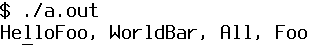
\includegraphics[width=0.5\textwidth]{data/demo21.png}
\end{figure}
\end{document}
